\documentclass[12pt]{article}
\usepackage[T2A]{fontenc}
\usepackage[utf8]{inputenc}
\usepackage[russian,english]{babel}
\usepackage[width=18cm,height=25cm]{geometry}
\usepackage{graphicx}
\usepackage{amsmath,amsfonts,amssymb}

\begin{document}
строчная формула $x=100$ \\%перенос на другую строку без абзаца, если просто пустрая строка то абзац
вынесенная формула
$$
\int_0^{\pi/2} dx\,\frac{1}{1+\tan^{2020}x}=?
$$
\begin{figure}
\centering
%\left   \right
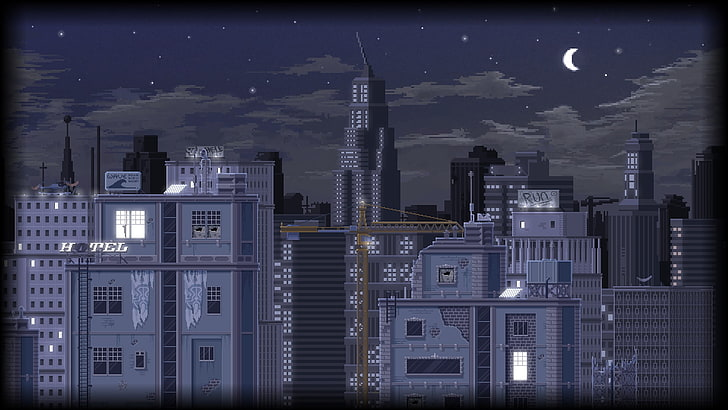
\includegraphics[width=0.7\textwidth]{the_last_lab/night.jpg}%path to the graph
\caption{picture}
\end{figure}
\section{название секции}%секции не нумеруются, еслиsection*{}
%\subsection
%\subsubsection

%table
\begin{table}%c l r-по центру, слева, справа |
\begin{tabular}{|c|c|r|}
\hline
ячуйка1& ячейка2 & ячейка3\\
\hline ячуйка1& ячейка8 & ячейка3\\
\hline ячуйка1& ячейка9 & ячейка3\\
\hline

\end{tabular}
\end{table}




\begin{table}[h!]%c l r-по центру, слева, справа |
\begin{tabular}{|p{10cm}|c|r|}
\hline
ячуйка1& ячейка2 & ячейка3\\
\hline ячуйка1& ячейка8 & ячейка3\\
\hline ячуйка1& ячейка9 & ячейка3\\
\hline

\end{tabular}
\end{table}


%matrix
$$\left(
\begin{array}{|c|c|c|}
1 & 2 & 3\\
4 & 5 & 6\\
7 & 8 & 9
\end{array}\right)
$$


$$
\begin{pmatrix}% vmatrix
1 & 2 & 3\\
4 & 5 & 6\\
7 & 8 & 9
\end{pmatrix}
$$
\end{document}